\documentclass[computationalMathematics.tex]{subfiles}

%%%%%%%%%%%%%%~~~~~~~~~~~~~~~~~~~~~~~~~~~~~~~~~~~~~~~~%%%%%%%%%%%%%%%
\chapter{5th of October 2018}
\chapterauthor{A. Frangioni}
%%%%%%%%%%%%%%~~~~~~~~~~~~~~~~~~~~~~~~~~~~~~~~~~~~~~~~%%%%%%%%%%%%%%%

\section{Unconstrained optimization}

Until now we stated that the best conditions for finding the optimum are encountered when the domain is a compact set and we have many derivatives.

Now we need to consider when we can stop our algorithm.

\begin{definition}[Unconstrained optimization problem]
We term \textbf{unconstrained optimization problem} the following
\[
(P)~f_* = \min \{f(\vect{x})~:~\vect{x} \in \R^n\}
\]
\end{definition}

In unconstrained optimization, we deal with an unbounded set ($\R^n$), hence Weierstrass theorem does not apply.
Because of this reason, we have no guarantee that a minimum $\vect{x}_*$ exists; moreover, provided its existence, finding it is an NP-hard problem. 
In order to make things easier, in practice we use a weaker condition: \textbf{local minimality}.

\begin{definition}[Local minimum]
Let $f: \R^n \to \R$. $\vect{x}_*$ is a \textbf{local minimum} if it is a global minimum in a ball around $\vect{x}^*$.
Formally, 
\[
  \min \{f(\vect{x})~:~\vect{x} \in \mathcal{B}(\vect{x}_*, \eps) \}
\]
for some $\eps > 0$.

Also, $\vect{x}^*$ is a \textbf{strict local minimum} if $f(\vect{x}) \,  {<} \, f(\vect{x}') ~ \forall \vect{x}' \in \mathcal{B}(\vect{x}_*, ~\eps)$.
\end{definition}

\begin{figure}[h]
  \centering
  \subfigure[Points where the derivative is not $0$.]{\includegraphics[width=0.35\textwidth]{pics/5ott/localopt1.pdf}\label{subfloat:5ott_1}}
  \hspace{0.5cm}
  \subfigure[Points where the derivative is $0$.]{\includegraphics[width=0.35\textwidth]{pics/5ott/localopt2.pdf}\label{subfloat:5ott_2}}\\
  \caption{Minima and not minima.}\label{fig:5ott_1}
\end{figure}

If $f'(\vect{x}) < 0$ or $f'(\vect{x}) > 0$, $\vect{x}$ clearly cannot be a local minimum, as shown in \Cref{fig:5ott_1}.

\subsection{First order model}

\recap{The first order model of $f$ is $L_{\vect{x}}(\vect{x}') = f(\vect{x}) + \nabla f(\vect{x}) (\vect{x}'-\vect{x})$, such that $\forall \vect{x}' \in \R^n$ close to $\vect{x}$ $f(\vect{x}') = L_{\vect{x}}(\vect{x}')  + R(\vect{x}'-\vect{x})$, where $R(\cdot)$ is called \textbf{residual} and it has the property of quadratic convergence: $\lim\limits_{\norm{h} \to 0} \frac{R(h)}{\norm{h}} = 0$.}

\begin{proposition}
Let $f$ be differentiable, if $\vect{x}$ is a local minimum, then $\nabla f(\vect{x}) = 0$.
\end{proposition}

In optimization, we are interested in moving towards a (local) minimum $\vect{x}_*$ as fast as possible.

\begin{proposition}\label{prop:step_dir}
	Let $f: \R^n \to \R$ be the objective function of the optimization problem (P) and let $\vect{x} \in \R^n$ be the current point at a generic iteration.
	In order to get closer to the optimum, we need to take a step along the \emph{anti-gradient} direction.
	Formally, $\vect{x}(\alpha) = \vect{x} - \alpha \nabla f(\vect{x})$, where $\alpha \in \R$ is called \emph{step size}.
\end{proposition}

\begin{proof}[Proof by contraddiction]
  Let us assume that $\vect{x}$ is a local minimum but $\nabla f(\vect{x}) \neq 0$.
  
  In our case, $\vect{x}' = \vect{x} -\alpha \nabla f(\vect{x})$, so let us plug it into the \emph{remainder version} of the Tailor's first-order model:
  \[
  \begin{split}
  	f(\vect{x}') &= \ps{\nabla f(\vect{x})}{\vect{x}' - \vect{x}} + f(\vect{x}) + R(\vect{x}' - \vect{x})\\
  	&= \ps{\nabla f(\vect{x})}{\vect{x} - \alpha \nabla f(\vect{x}) - \vect{x}} + f(\vect{x}) + R(\vect{x} - \alpha \nabla f(\vect{x}) - \vect{x})\\
  	&= \ps{\nabla f(\vect{x})}{- \alpha \nabla f(\vect{x})} + f(\vect{x}) + R(- \alpha \nabla f(\vect{x}))\\
  	&= f(\vect{x}) - \alpha \norm{\nabla f(\vect{x})}^2 + R(- \alpha \nabla f(\vect{x}))
  \end{split}
  \]
   
	Once we fixed the moving direction, we can choose the step size $\alpha$, so it can be proved that $\lim\limits_{\alpha \to 0} \frac{R(- \alpha \nabla f(\vect{x}))}{\norm{\alpha \nabla f(\vect{x})}} = 0$, that is equivalent by definition to $\forall \eps > 0 \, \exists \bar{\alpha} > 0$ s.t. $\frac{R(- \alpha \nabla f(\vect{x}))}{\alpha \norm{\nabla f(\vect{x})}} \leq \eps~\forall ~ 0 \leq \alpha < \bar{\alpha}$.

 	If we take $\eps < \norm{\nabla f(\vect{x})}$, we get  $R(- \alpha \nabla f(\vect{x})) < \alpha \norm{\nabla f(\vect{x})}^2$, then 
	\[
	  f(\vect{x}(\alpha)) = f(\vect{x}) - \alpha \norm{\nabla f(\vect{x})}^2 + R(- \alpha \nabla f(\vect{x})) < f(\vect{x})
	\]
	$\forall \alpha < \bar{\alpha}~\vect{x}$ cannot be a local minimum.
\end{proof}

\Cref{prop:step_dir} states that the first order model allows to find the decreasing direction, but if the gradient is $0$ we do not know if we are in presence of a minimum, maximum or a saddle point.
To discriminate among those, we exploit the information provided by the second derivative.

\subsection{Second order model}

\begin{proposition}\label{fact:5ott_1}
Let $f: \R^n \to \R$ such that $f \in C^2$.
If $\vect{x}$ is a local minimum then the gradient is positive semidefinite.
Formally, $\nabla^2 f(\vect{x}) \succeq 0$.
\end{proposition}

\begin{proof}[Proof by contraddiction]
  Our contradictory hypothesis is that we are in a local minimum, but the Hessian is not positive semidefinite, there there is a direction $\vect{d} \in \R^n$ of negative curvature.
  Formally, $\exists \vect{d}$ s.t.~$\vect{d}^T \nabla^2 f(\vect{x}) \vect{d} < 0$ or equivalently, the Hessian has a negative eigenvalue $\lambda_i <0$.
  
  Let us consider that $\vect{d}$ has norm $1$ without loss of generality and let us be given a step $\vect{x}(\alpha) = \vect{x}+ \alpha \vect{d}$ and then take the second-order Taylor formula as follows (where there is no linear term involved because $\nabla f(\vect{x}) = 0$):
	
\[
	\begin{split}
		f(\vect{x}(\alpha)) &= f(\vect{x}) + \frac{1}{2} \tr{(\alpha \vect{d})} \nabla^2 f(\vect{x}) (\alpha \vect{d}) + R( \vect{x}(\alpha) - \vect{x})\\
  		f(\vect{x}(\alpha)) &= f(\vect{x}) + \frac{1}{2} \alpha^2 \vect{d}^T \nabla^2 f(\vect{x}) \vect{d} + R( \alpha \vect{d} )
  \end{split}
\]
with $\lim\limits_{\norm{h} \to 0} \frac{R(h)}{\norm{h}^2} = \lim\limits_{\alpha \to 0} \frac{R(\alpha \vect{d})}{\alpha^2} = 0$ or equivalently $\forall \eps > 0 \, \exists \bar{\alpha} > 0$ s.t. $R(\alpha \vect{d}) \leq \eps \alpha^2 ~ \forall 0 \leq \alpha < \bar{\alpha}$.

At this point, since this condition holds for each $\eps$ we are allowed to take the most convenient: $\eps < -\frac{1}{2} \vect{d}^T \nabla^2 f(\vect{x}) \vect{d}$, so that we obtain this condition on the residual $R(\alpha \vect{d}) < -\frac{1}{2} \alpha^2 \vect{d}^T \nabla^2 f(\vect{x}) \vect{d}$, hence
\[
f(\vect{x}(\alpha)) = f(\vect{x}) + \frac{1}{2} \alpha^2 \vect{d}^T \nabla^2 f(\vect{x}) \vect{d} + R(\alpha \vect{d}) < f(\vect{x}) \forall \, 0 \leq \alpha < \bar{\alpha}
\]

The contraddiction lies in the fact that $\vect{x}(\alpha)$ leads to a value of $f$ smaller than the one in $\vect{x}$.
\end{proof}

\Cref{fact:5ott_1} states that a positive semidefinite Hessian is a necessary condition for a local minimum.
Follows a proposition that gives a sufficient condition.

\begin{proposition}
  Let $f: \R^n \to \R$ s.t. $f \in C^2$ and let the Hessian be symmetric (hence real eigenvalues).
  If $\nabla f(\vect{x}) = 0$ and the Hessian is strictly positive definite ($\nabla^2 f(\vect{x}) \succ 0$) then $\vect{x}$ is a local minimum.
\end{proposition}

\begin{proof}
$\vect{x} \in \R^n$ is a point where the gradient of the function is $0$ we get the following second order Taylor approximation for $\vect{x}_{\text{new}} = \vect{x} + \vect{d}$ (unitary step size for simplicity):

\[
  f(\vect{x} + \vect{d}) = f(\vect{x}) + \frac{1}{2} \vect{d}^T \nabla^2 f(\vect{x}) \vect{d} + R(\vect{d})\mbox{ with } \lim\limits_{h \to 0} \frac{R(\vect{d})}{\norm{\vect{d}}^2} = 0
\]
  Hence, by definition of limit $\forall \eps > 0~\exists~\delta > 0$ s.t. $R(\vect{d}) \leq \eps \norm{\vect{d}}^2~\forall \vect{d} \in \R^n$ s.t. $\norm{\vect{d}} < \delta$.

Since the Hessian is strictly positive definite, the smallest eigenvalue $\lambda_{\text{min}}$ is strictly greater than $0$, hence the variational characterization of eigenvalues $\vect{d}^T \nabla^2 f(x) \vect{d} \geq \lambda_{\text{min}} \norm{\vect{d}}^2$.

\todo[inline]{Aggiungere la ref alla variational characterization nella parte di Numerical Methods}
  We are now ready to pick the $\eps$ we prefer ($\eps < \lambda_{\text{min}}$) to get $\forall \vect{d}$ s.t. $\norm{\vect{d}} < \delta$
\[
  f(\vect{x} + \vect{d}) = f(\vect{x}) + \frac{1}{2} \vect{d}^T \nabla^2 f(\vect{x}) \vect{d} + R(\vect{d}) \geq f(\vect{x}) + (\lambda_{\text{min}} - \eps) \sqrnorm{\vect{d}} > f(\vect{x})
\]

  The term $\lambda_{\text{min}} - \eps$ is strictly positive.
\end{proof}

\noindent In the rest of this lecture, we will provide conditions that ensure that once a local minimum is found, it is also a global minimum.

So far, we said that the local minima are those points where the gradient is $0$ and the Hessian is positive semidefinite.
An easy way to ensure that the Hessian is positive semidefinite in a ball around $\vect{x}$ is to have that the Hessian is positive semidefinite everywhere ($\forall \vect{x} \in \R^n$) and this is guaranteed to be true whenever $f$ is a convex function.

\section{Convexity}
Let us introduce convexity as far as both sets and functions are concerned.

\subsection{Convex sets}

\begin{definition}[Convex hull]
  Let $\vect{x}, \vect{y} \in \R^n$ we term \textbf{convex hull} and denote conv$(\vect{x}, \vect{y}) = \{\vect{z} = \alpha \vect{x} + ( 1 - \alpha )\vect{y}~:~ \alpha \in [0, 1]\}$ the segment joining $\vect{x}$ and $\vect{y}$.
\end{definition}

\begin{definition}[Convex set]
  Intuitively, we say that $C$ is a \textbf{convex set} if for each couple in the set, the line joining such points belongs to the set.

  \noindent Formally, $C \subset \R^n$ is a \textbf{convex set} if $\forall~\vect{x}, \vect{y} \in C$ conv$(\vect{x},\vect{y}) \subseteq C$.
\end{definition}

\noindent Notice that ``disconnected sets'' cannot be convex sets.

\begin{definition}[Convex hull of a set]
Given a set $S \subseteq \R^n$, we can ``complete'' it to a convex set conv$(S)$, called \textbf{convex hull of $S$}:
\[
\begin{array}{rcl}
 conv(S) & = &
 \bigcup \{ \, conv(\vect{x},\vect{y}) \,:\, \vect{x}, \vect{y} \in S \, \} \\[0.2cm]
 & = &
 \bigcap \{ \, C \,:\, C \mbox{ is convex } \wedge
                         C \supseteq S \, \}
\end{array}
\]
Equivalently, the convex hull of $S$ can be defined iteratively as the convex hull of all the couples of points in $S$.

\noindent Equivalently, we can define the convex hull of a set $S$ as the smallest convex set containing $S$.
\end{definition}

\begin{myframe}{\bf Note}
	A more general definition of a convex hull is the following:
	conv$(\{\vect{x}_1, \ldots, \vect{x}_k\}) = \{\vect{x} = \sum\limits_{i=1}^k \alpha_i \vect{x}_i~:~\sum\limits_{i=1}^k \alpha_i = 1,~\alpha_i \geq 0~\forall i\}$ 
\end{myframe}

\begin{definition}[Unitary simplex]
	We term \textbf{unitary simplex} the set of $k$ non-negative scalars summing to $1$, formally
	\[
	\Theta^k = \{\sum\limits_{i=1}^k \alpha_i \vect{x}_i\in \R^k~:~\sum_{i=1}^k \alpha_i = 1, \alpha_i \geq 0~\forall i\}
	\]
\end{definition}

\begin{figure}[h]
	\centering
	\subfigure[In $\R^2$]{\includegraphics[width=0.35\textwidth]{pics/5ott/usR2.png}\label{subfloat:5ott_3}}
	\hspace{0.5cm}
	\subfigure[In $\R^3$]{\includegraphics[width=0.35\textwidth]{pics/5ott/usR3.png}\label{subfloat:5ott_4}}\\
	\caption{Example of unitary simplexes.}\label{fig:5ott_2}
\end{figure}

\noindent Our goal is to find the simplest possible convex set that approximates our set.

\begin{proposition}
A convex set is equal to its convex hull. 
Formally,
\[
	C \text{ is convex } \iff C = \text{conv}(C)
\]
\end{proposition}

We are interested in sufficient conditions for convexity.

\begin{definition}[Cone]
  We term \textbf{cone} the set $\mathcal{C} = \{\vect{x} \in \R^n ~:~\alpha \vect{x} \in \mathcal{C}\forall\alpha \geq 0\}$.
\end{definition}

\noindent An attentive reader may notice that the definition of cone is a relaxation of the unitary simplex, where we do not require the unitary sum.

\begin{example}
	The following sets are convex:
	\begin{itemize}
		\item Convex polytope $conv( \, \{\vect{x}_1, \ldots, \vect{x}_k\} \, )$, unitary simplex $\Theta$
		\item Affine hyperplane: $\mathcal{H} := \{ \vect{x} \in \R^n~:~\tr{vect{a}} \vect{x} = b \}$
		\item Affine close (open) subspace: $\mathcal{S} := \{\vect{x} \in \R^n~:~ \tr{\vect{a}} vect{x} \leq (<) b\}$
		\item Close (open) ball of radius $r$ in $p$-norm, $p \geq 1$: $\mathcal{B}_p(\vect{x}, r) = \{ \vect{y} \in \R^n ~:~ \norm{\vect{y} - \vect{x}}_p \leq (<) r \}$
		\item Close (open) ellipsoid: $\mathcal{E}(Q,\vect{x},r) := \{y \in \R^n~:~\tr{(y - \vect{x})}Q(y - \vect{x}) \leq (<) r\}$  with $Q \succeq 0$.
			Notice that ellipsoids are levelsets of quadratic functions.
		\item Cones
		\item Conical hull of a finite set of directions: 
		\[
			cone(\{\vect{d_1}, \ldots, \vect{d_k}\}) = \Big\{ \vect{d} = \sum\limits_{i=1}^k \mu_i \vect{d_i}~:~\mu_i \geq 0~\forall \, i \, \Big\}
		\]
		\item Lorentz's cone (ice-cream cone): $\mathbb{L} = \Big\{ \, \vect{x} \in \R^n \,:\, \vect{x}_n \geq \sqrt{\sum_{i=1}^{n-1} \vect{x}_i^2} \, \Big\}$
		\item Cone of positive semidefinite matrices: $\mathbb{S}_+ = \{ \, A \in \mathcal(M)(n, \R^n) ~:~ A \succeq 0\}$
	\end{itemize}
\end{example}

\begin{proposition}
The following operations preserve convexity.
\begin{enumerate}
	\item Given a possibly infinite family of convex sets (${\{C_i\}}_{i \in I}$), the intersection ($\bigcap_{i \in I} C_i$) is convex;
	\item If we have convex sets in different subspaces, their Cartesian product is a convex set ($C_1, \ldots, C_k$ convex $\iff C_1 \times \cdots \times C_k$ convex);
	\item Given a convex set, its image under a linear mapping (i.e. scaling, translation, rotation) is a convex set.
	Formally, let $C$ be a convex set. Then $A(C) := \{\vect{x} = A\vect{y} + \vect{b}~:~\vect{y} \in C\}$ for a given $A \in \mathcal{M}(n, \R)$ and $\vect{b} \in \R^n$ is convex; 
	\item If $C$ is a convex set its inverse image under a linear mapping is convex as well.
	Formally, $A^{-1}(C) := \{x~:~Ax + b \in C\}$ is convex; 
	\item Let $C_1$ and $C_2$ convex and let $\alpha_1, \alpha_2 \in \R$. Then $\alpha_1 C_1 + \alpha_2 C_2 := \{ \vect{x} = \alpha_1 \vect{x}_1 + \alpha_2 \vect{x}_2 \,:\, \vect{x}_1 \in C_1, \vect{x}_2 \in C_2\}$ is convex;
	\item Let $C \subseteq \R^{n_1} \times \R^{n_2}$ be a convex set. Slicing and projection lead to convex sets as well, as shown in \Cref{fig:5ott_3}:
	\begin{description}
		\item[{\small \sc Slice:}] $C_s(\vect{y}) := \{\vect{x} \in \R^{n_1}~:~(\vect{x}, \vect{y}) \in C\}$ is convex
		\item[{\small \sc Projection:}] $C_p := \{\vect{x} \in \R^{n_2}~:~\exists \vect{y}$ s.t. $(\vect{x}, \vect{y}) \in C\}$ is convex
	\end{description}
	\item Given a convex set $C$, the interior of such set and its closure are convex.
\end{enumerate}
\end{proposition}

\begin{figure}[h]
  \centering
  \subfigure[Slice on $\bar{\vect{y}}$]{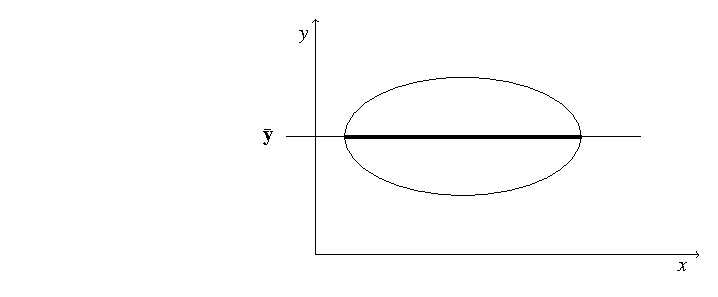
\includegraphics[width=0.45\textwidth]{tikzpics/slice.pdf}\label{subfloat:5ott_5}}
  \hspace{0.5cm}
  \subfigure[Project on the $x$ component]{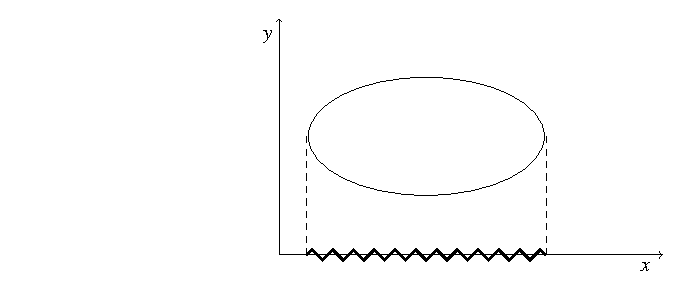
\includegraphics[width=0.45\textwidth]{tikzpics/project.pdf}\label{subfloat:5ott_6}}\\
  \caption{Pictorial examples of slicing and projecting.}\label{fig:5ott_3}
\end{figure}

\begin{theorem}
  $\mathcal{P}$ is a polyhedron iff any of its points can be written as a combination of a point in a convex set and one in a cone.
  Formally, iff $\exists \{\vect{x}_1, \ldots, \vect{x}_k\} \subseteq \R^n$ and $\{\vect{d}_1, \ldots, \vect{d}_h\} \subseteq \R^n $ s.t. $\mathcal{P} = conv(\{\vect{x}_1, \ldots, \vect{x}_k\}) + \text{cone}(\{d_1, \ldots, d_h\})$.
\end{theorem}

\noindent Notice that whenever we are interested in proving that a set with a certain shape is convex, we could try to derive it from an object that we know is convex through the operations we enumerated above.

\subsection{Convex functions}

In the rest of this lecture we will introduce the class of convex functions, that have the characteristic of having local minima coinciding with global minima.

\begin{definition}[Graph]
	Let $f: \R^n \to \R$, we term \textbf{graph} of $f$ the set of ordered pairs $(\vect{x}, y)$ such that $f(\vect{x}) = y$.
\end{definition}

\begin{definition}[Epigraph]
	Let $f: \R^n \to \R$, we term \textbf{epigraph} or \textbf{supergraph} of $f$ the set of points lying on or above its graph.
	Formally,
	\[
	\text{epi}(f)= \{(\vect{x},\mu )~:~\vect{x}\in \R^n,~ \mu \in \R,~\mu \geq f(\vect{x})\} \subseteq \R ^{n+1}
	\]
\end{definition}

\begin{definition}[Convex function]
  Let $f:\R^n \to \R$ be a function. We say that $f$ is \textbf{convex} if $\forall\vect{x}, \vect{y} \in \R^n$, the segment that joins $f(\vect{x})$ and $f(\vect{y})$ lies \emph{above} the function.

  \noindent In other words, $f$ is \textbf{convex} iff $epi(f)$ is convex.

  \noindent Equivalently, we say that $f$ is \textbf{convex} if $\forall \vect{x}, \vect{y} \in dom(f)$ for any $\alpha \in [0, 1]$, $\alpha f(\vect{x}) + (1-\alpha) f(\vect{y}) \geq f(\alpha \vect{x} + (1-\alpha)\vect{y})$.

  \noindent Equivalently, $\forall \vect{x}^1$, \ldots, $\vect{x}^k$, $\alpha \in \Theta^k$
\[
 f \left( \sum_{i=1}^k \alpha_i \vect{x}^i \right) \leq \sum_{i=1}^k \alpha_i f(\vect{x}^i)
\]
\end{definition}

\begin{definition}[Strict convexity]
	Let $f: \R^n \to \R^m$. We term $f$ \textbf{strictly convex} iff $\alpha f(\vect{x}) + (1 - \alpha) f(y) > f(\alpha \vect{x} + (1 - \alpha) y )$.
\end{definition}

\begin{definition}[Concave function]
	Let $f:\R^n \to \R$ be a function. We say that $f$ is \textbf{concave} if $\forall\vect{x}, \vect{y} \in \R^n$, the segment that joins $f(\vect{x})$ and $f(\vect{y})$ lies \emph{below} the function.
	Formally, $\forall \vect{x}, \vect{y} \in dom(f)$ for any $\alpha \in [0, 1]$, $\alpha f(\vect{x}) + (1-\alpha) f(\vect{y}) \leq f(\alpha \vect{x} + (1-\alpha)\vect{y})$.
\end{definition}

\begin{definition}[Sublevel graph]
  Let $f: \R^n \to \R^m$ be a function. We term \textbf{sublevel graph} of $f$ on a scalar $v \in \R$ and denote $S(f, v)$ the projection on the $\vect{x}$ axis of the portions of the graph of $f$ which lie below the constant value $v$.
\end{definition}

\addpic{0.7}{tikzpics/sublevel.pdf}{$f(x) = {x}^5 - 8 {x}^3 +10x +15$ in blue and its sublevel graph in orange.}{fig:5ott_4}

\begin{proposition}\label{prop:5ott_1}
The following holds:
\begin{itemize}
 \item Let $f$ convex. Then $S(f,v)$ is convex $\forall v \in \R$;
 \item $f$ is concave if $-f$ is convex.
\end{itemize}
\end{proposition}

\mantra{Convex analysis is a one-sided world.}

The second statement of \Cref{prop:5ott_1} is useful to make a comparison between minimizing and maximizing. In particular, if our aim is to maximize the function, we can be sure to have found a global maximum if the function is concave.

\begin{definition}[Strong convexity]
  Let $f: \R^n \to \R$.
  We term $f$ \textbf{strongly convex modulus} a scalar $\tau > 0$ iff $f(\vect{x}) - \frac{\tau}{2}\,\norm{\vect{x}}^2$ is convex.
  
  Formally,
 \[
   \alpha f(\vect{x}) + (1 - \alpha) f(\vect{y}) \geq f(\alpha \vect{x} + (1 - \alpha) \vect{y})+ \frac{\tau}{2} \alpha (1 - \alpha) \norm{(\vect{y} - \vect{x})}^2
 \]
\end{definition}

In the next lecture we will provide techniques that allow to check if a function is convex in practice.
